%% ----------------------------------------------------------------
\chapter{Introduction (ab)}
%% ----------------------------------------------------------------

\section{Description of Problem}

This project seeks to produce a system that is able to interface a camera with an autopilot on board an Unmanned Aerial Vehicle (UAV). The desired module must capture a digital still image from the camera, then transmit this data via a low-bandwidth serial link to the autopilot. The autopilot then re-transmits this data over its wireless (RF) link to a ground station running our customers ground software. Then our customer's software provides a TCP/IP interface, which allows us to capture this data in our own program, and then display the captured image data to the user. Both the Autopilot and our customer's ground station software currently exist.

\begin{figure}[H]
        \centering
        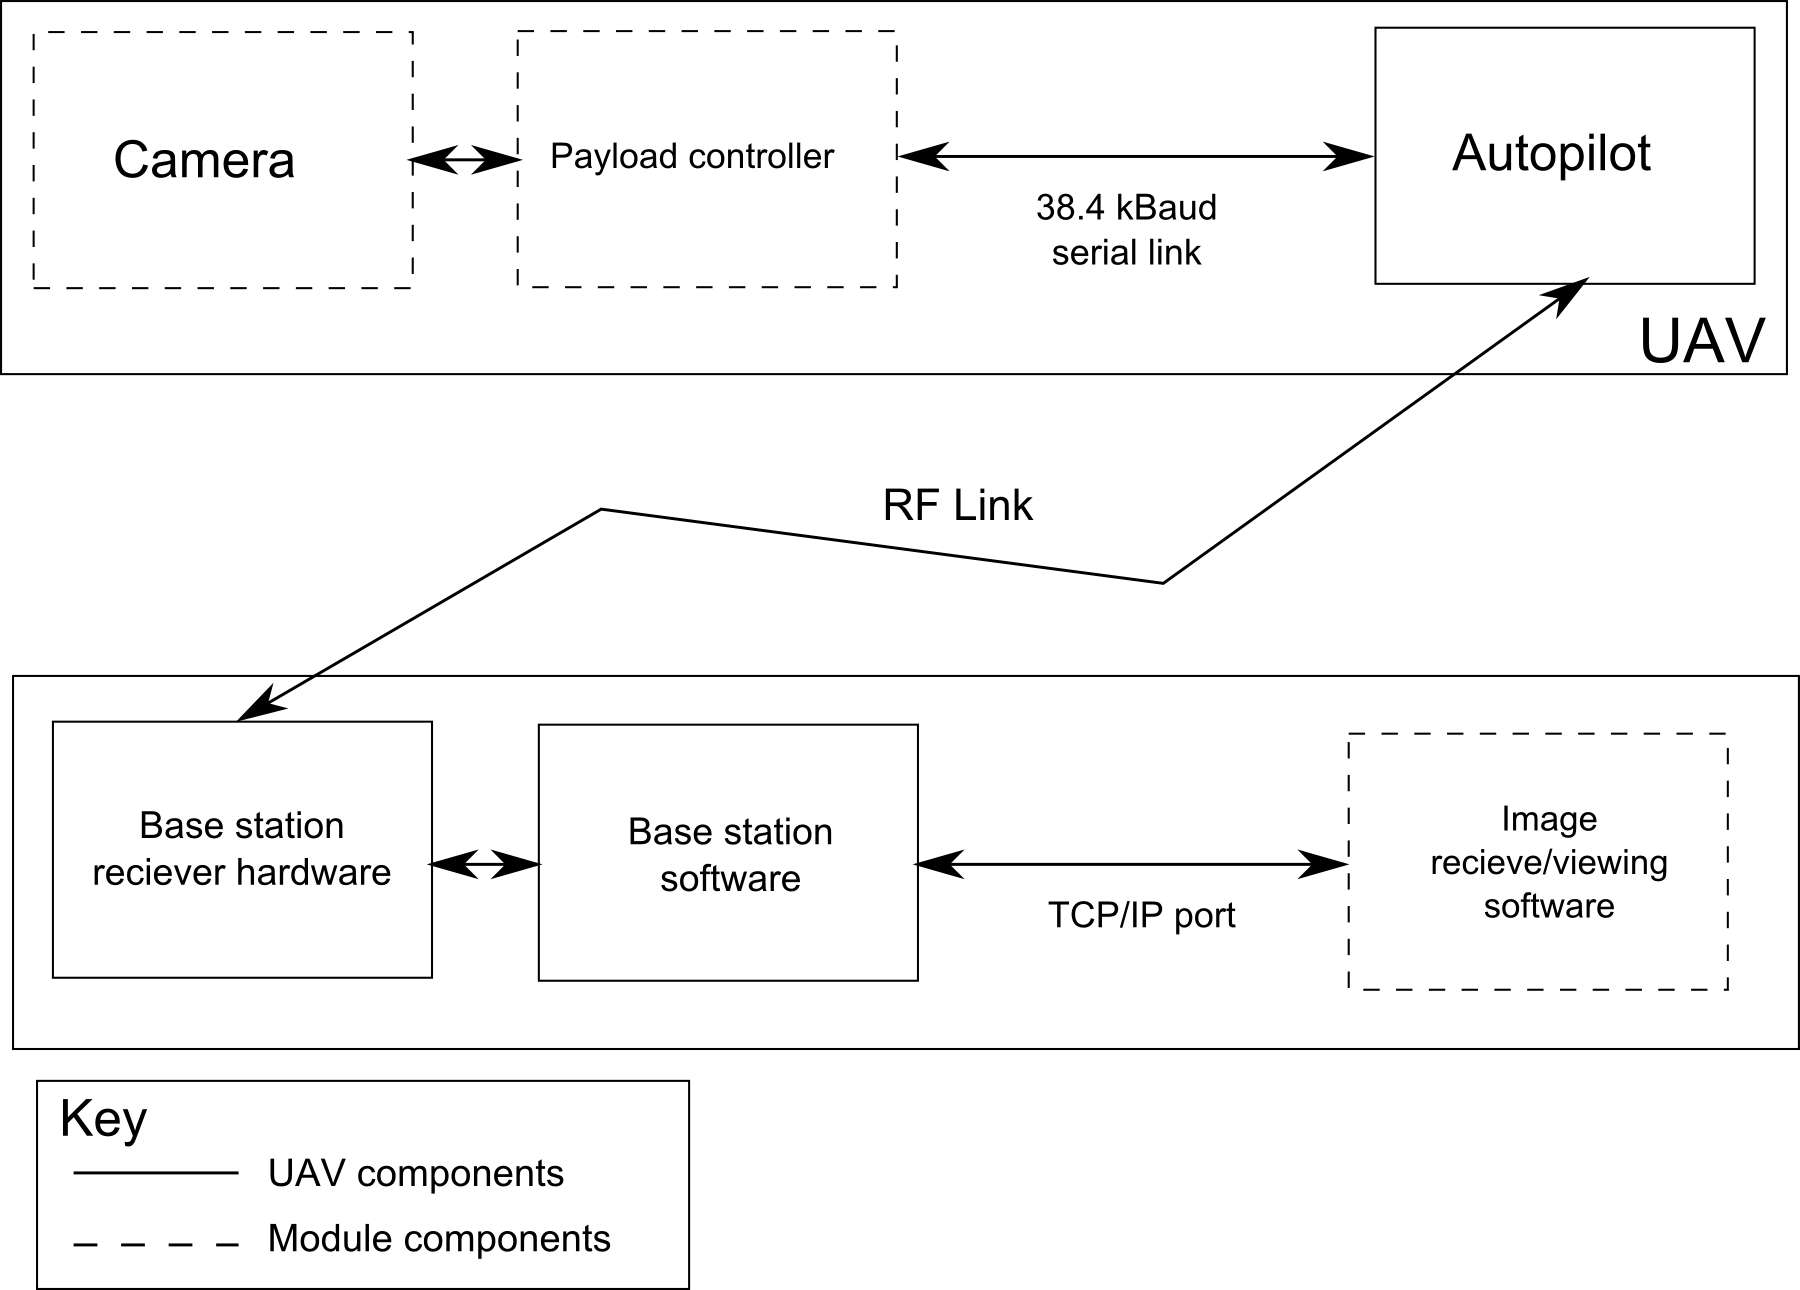
\includegraphics[width=1.00\textwidth]{figures/spec_block_diagram_2.png}
        \captionof{figure}{Block diagram displaying how the separate parts of this project interact, and which parts of this project we need to implement.}
        \label{fig:blockDiagram}
\end{figure}

Deliverables for this project would be a suitable camera for the project, an electronic module presented (preferably) on PCB, and an additional piece of ground station software to interact with the payload module. It needs to be in a state such that it would require minimal additional work before being presented to the clients of our customer as a potential "Wireless Camera Payload" solution that they would be able to implement. Therefore, delivery of User Documentation, and a repository containing all hardware and software necessary to easily reproduce the project is required.

\subsection{SkyCircuits}

SkyCircuits Ltd. \cite{SkyCircuits} is a company that designs and sells autopilot modules and ground station software for unmanned aircraft. These modules are able to take control of a UAV from take-off to landing, along a user-defined path, with no need for human intervention. SkyCircuits market two different autopilots: A more expensive model aimed at the recreational, academic and commercial markets, and a cheaper, less powerful module, aimed at the Recreational market only.

It was this company's autopilot module that recently successfully flew the world's first 3D-printed UAV, the Southampton University Laser Sintered Aircraft (SULSA), \cite{SULSA} an event which was also covered by the media \cite{SC_Press}.

Our contact from SkyCircuits for this project is its director, Dr. Matt Bennett.

\section{Existing Solutions}
\label{sec:existing_soln}

Currently, SkyCircuits' customers have implemented a system where they have retrofitted a high-resolution camera to a UAV, but this acts entirely independently of the autopilot module, and images are stored locally, therefore there is no way of knowing whether an image taken during flight is any good. The camera used for this system is very expensive (approximately \pounds 2000). The system we present in this project is significantly cheaper than this existing setup.

\section{Project Motivation}

The cost and inflexibility of the existing solution \ref{sec:existing_soln} means that it is unlikely that recreational users will want to replicate this system. Creating a camera payload for the autopilot that is cheaper, more functional (in that it would be able to exploit the wireless link furnished by the autopilot), and open source, is in our customer's interest as it may be useful in furthering interest around their products.

Also, this project serves to test a key piece of functionality of the autopilot modules to its limit - the payload module port. This project serves to test the robustness of this feature, and help iron out any potential bugs, and encourage development of further payload modules. The ability to further develop this project to include other types of payload and further potential applications of the autopilot would potentially increase interest around the products.

Both of the autopilot modules marketed by SkyCircuits Ltd. offer the "payload" feature.

\section{Solution}

Our solution, presented in Chapter \ref{chap:implementation}, comprises acomplete system implemented on PCB, connected to a UAV-mountable board camera, which, when prompted by our software, is able to capture an image, store it locally on an SD card, then send it over the wireless link provided by the autopilot module to a "ground station" (a laptop configured with the autopilot's wireless receiver and SkyCircuits' software). Our software interacts with the existing software's TCP/IP port, and can send images via the autopilot to the payload, and accept data from the payload and display it on screen.

\section{Report Structure}

Below is a short summary of what each section of this report contains:

\subsection{Background Research}
This section introduces various topics that have been relevant to this project, including:
\begin{itemize}
\item Image Compression Theory
\item JPEG Image Compression 
%\item Automatic Repeat Requests
%\item Parity Bits
%\item ZigBee modules
%\item SkyCircuits Autopilot System
\end{itemize}

\subsection{Specification}
The specification in its submitted form, along with justification for the inclusion of each point.

\subsection{Planning}
Our project plan, including our initial Gantt Chart, Risk Analysis, Skills Audit, Work Allocation, Planned Communication, Resources, Milestones and Technical Plan.

\subsection{Design Choices}
This section explains the various design choices which we have made during this project, including a discussion of the other options that were available to us at the time, and a justification for our choice.

%%...more to follow when report structure is a bit more concrete...

\section{Authorship}

The main author of each section of this report is indicated by initials in 
the title of either the chapter, section, subsection, etc. that the author 
was responsible for writing. Editing the report was the entire group's 
responsibility.

\begin{itemize}
\item ab - Andrew Busse
\item jc - John Charlesworth
\item mh - Micheal Hodgson
\item ms - Paramithi "Mitch" Svastisinha
\item ps - Piyabhum Sornpaisarn
\end{itemize}
